\appendix
\section{Collaborative Writing Evidence}
\label{app:collab}

The technical-report rubric (Lecture 11, slide 14) requires the report
to ``show evidence of collaborative writing, not just a final PDF.''
Two artefacts are reproduced here: an Overleaf history snapshot showing
all three authors' colored edit ranges across multiple revisions, and
the project repository's \texttt{git log} restricted to the
\texttt{report/} subtree.

\begin{figure}[htbp]
\centering
% TODO: replace with screenshot from Overleaf -> File -> History
\includegraphics[width=\columnwidth]{figures/overleaf_history.png}
\caption{Overleaf history panel. Each author's edits are rendered in
  a different color. Window covers the period from
  the first \texttt{report/main.tex} commit to the final submission
  on 05/07.}
\label{fig:overleaf-history}
\end{figure}

\begin{figure}[htbp]
\centering
% TODO: replace with terminal screenshot from
%   git log --pretty=format:'%h %an %ad %s' -- report/
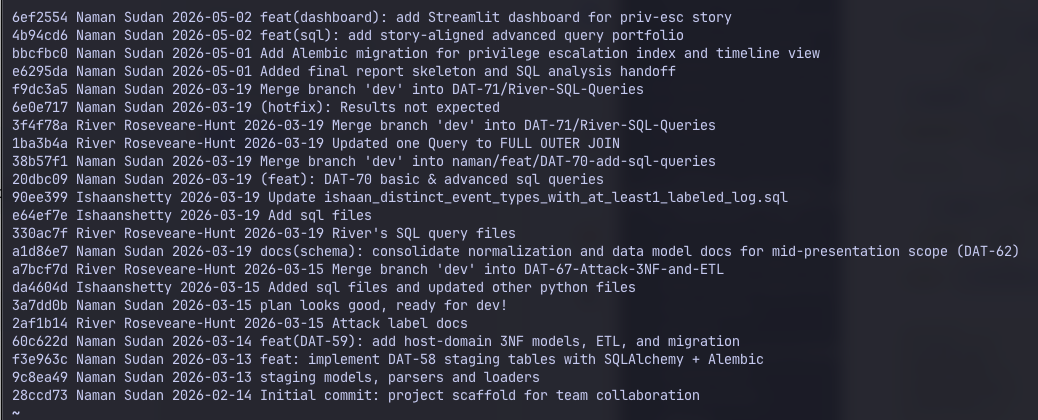
\includegraphics[width=\columnwidth]{figures/git_log_report.png}
\caption{\texttt{git log} restricted to \texttt{report/}. Shows
  contributions from all three authors.}
\label{fig:gitlog-report}
\end{figure}

\section{Repository Map}
\label{app:repo}
The full project repository (frozen at the commit referenced on
Canvas) is laid out as follows:

\begin{verbatim}
data-201-security-log-analysis/
|-- README.md             setup + run + dashboard instructions
|-- docker-compose.yml    Postgres 16
|-- alembic/              schema migrations
|-- src/
|   |-- models/           SQLAlchemy ORM models
|   |-- parsers/          raw log parsers
|   |-- loaders/          ETL pipelines
|   `-- dashboard/        Streamlit app (Section 7)
|-- sql/
|   |-- 3nf/              per-table CREATE TABLE
|   |-- 3nf/_indexes.sql  performance indexes (Section 6.3)
|   |-- 3nf/_views.sql    persisted views (v_attack_timeline)
|   |-- queries/basic/    six basic queries (B1-B6)
|   `-- queries/advanced/ seven advanced queries (A1-A7)
|-- notebooks/            10 exploration notebooks (mid-pres)
|-- docs/
|   |-- schema/           data_model_3nf.md, normalization_raw_to_3nf.md
|   |-- er_diagrams/      drawio sources + exported PDF
|   `-- data_exploration/ per-source findings docs
|-- presentation/         mid-pres + final pres decks
`-- report/               this report (LaTeX sources)
\end{verbatim}
